\section{Evaluation}
\label{sec:eval}

Although \quicksand~presents Iterative Deepening and data-race PPs as interconnected techniques, they each could theoretically be employed alone in other model checkers.
For example, a single-state-space tool could use data-race candidates during immediately subsequent interleavings, essentially changing the state space on the fly.
Likewise, a message-passing-only tool could employ Iterative Deepening despite data races being absent from its concurrency model.
Hence, though many of our experiments compare \quicksand~to the state-of-the-art as a whole,
we also sought to evaluate each technique individually.
Our evaluation answers the following questions:
\begin{enumerate}

	\item Does \quicksand~improve upon state-of-the-art MC?
		\begin{enumerate}
			\item Does Iterative Deepening find bugs faster
				%than SSS-MC
				in subset state spaces, even without data-race PPs?
			% Probably not... ICB is state of the art here.
			% In large tests, can Iterative Deepening provide partial verification by completing smaller state spaces
			\item Do data-race PPs expose new bugs that couldn't be found with SSS-MC's fixed-PP-set approach?
				% Elaborate later:
				% Among those, how many were missed in a {\em completed} execution of the otherwise ``maximal'' state space?
		\end{enumerate}
	\item Does MC improve the accuracy of data-race detection?
		\begin{enumerate}
			\item Do we avoid false positives compared to a single-execution data race analysis?
				% Explain later as:
				% How many data-race candidates were verified as benign
				% But to be fair, you have to count how many DRs are reported as "couldn't test these, check yourself" at the end.
				% Also Include:
				% How many false positives does the free-re-malloc technique suppress?
				% to do (done) If you have time, re-run all of the dr-only bug tests, with DR_FALSE_NEG enabled, and see how much fewer bugs get found (how many bugs get pushed past the time limit?)
				% Answer: Just 1. (for p2s at least; as of time of writing, pintos dr-falsenegs not run yet)
			\item Do we find data-race bugs that would be false-negatives during a single-execution analysis?%Do we avoid false negatives compared to single-pass?
		\end{enumerate}
\end{enumerate}

%%%%%%%%%%%%%%%%%%%%%%%%%%%%%%%%%%%%%%%%%%%%%%%%%%%%%%%%%%%%%%%%%%%%%%%%%%%%%%%%

\subsection{Test Suite}
Our test suite consists of \numthrlibs~``P2'' student thread libraries, from CMU's 15-410 OS class,
and \numpintoses~``Pintos'' student kernels, from Berkeley's CS162 and U. Chicago's CS230 OS classes.
%
The P2 thread library comprises \texttt{thr\_create()}, \texttt{thr\_exit()}, \texttt{thr\_join()}, mutexes, condition variables, semaphores, and r/w locks;
all implemented from scratch in userspace with a UNIX-like system call interface \cite{kspec,thrlib}.
%
The Pintos kernel project
involves implementing priority scheduling, \texttt{sleep()}, and user-space process management (\texttt{wait()} and \texttt{exit()})
using provided bare-bones mutex, context-switch, and virtual memory implementations
\cite{pintos}.
% P2 SLOC stats: 1807 avg; 1723 median; range 1181-4114.
% All numbers, obtained with:
% cd p2s; for i in */*; do wc -l $i/user/libthread/*.{c,h,S} $i/user/libthread/*/*.{c,h,S} ; done | grep total
% 1181 1192 1221 1230 1238 1240 1243 1261 1275 1307 1310 1318 1325 1334 1336 1345 1366
% 1388 1388 1403 1415 1416 1430 1451 1478 1498 1527 1589 1618 1635 1638 1654 1675 1676
% 1716 1719 1720 1723 1723 1727 1737 1743 1744 1751 1769 1777 1782 1789 1789 1812 1918
% 1926 1946 1994 2022 2043 2066 2077 2088 2099 2131 2164 2172 2190 2215 2227 2277 2282
% 2384 2387 2483 2486 2503 2514 2551 2597 2610 2665 4114
Though not ``real world'' programs, both projects are quite complex:
the P2s average 1807 lines of code,%C and x86 assembly (stddev 489.5),
% Pintos SLOC stats: 718.1923077 avg; 643 median; range 68-1821
% Obtained with:
%function getloc {
%	diff -ru /tmp/shit/pintoses/di/src/$2/ $1/src/$2 | diffstat | grep insertions | sed 's/.*changed, //' | sed 's/ insertion.*//'
%}
%for i in `ls -d /tmp/shit/pintoses/* | grep -v -- "-p1$"`; do
%#for i in /tmp/shit/pintoses/daniel-deniz*; do
%	echo -ne "$i";
%	tloc=`getloc $i threads`
%	uloc=`getloc $i userprog`
%	dloc=`getloc $i devices`
%	echo -e "\t$tloc\t$uloc\t$dloc"
%done
and the Pintoses average 718.

We chose P2s and Pintoses for our test suite because of the relative ease of generating hundreds of unique state spaces,
varied in size and correctness, and with a diverse set of bug types\footnote{
Many of the codebases exhibited {\em deterministic} bugs (i.e., encountered on the first interleaving tested).
We fixed these by hand in advance to ensure that every bug in our study required some meaningful work by the MC.}.
% TODO: Is this ok? Too arrogant?
We believe that merely finding a small handful of new real-world bugs is too anecdotal,
and that our test suite's size allows for a more statistically significant comparison among MC and data-race testing strategies,
%compared to anecdotally showing a small handful of new bugs that could be found in real-world programs.

\newcommand\mxtest{\texttt{mx\_test}} % TODO: find a way to change name to mutex_test without overflowing lines in the next paragraph
\newcommand\tej{\texttt{join\_test}}
\newcommand\bct{\texttt{bcast\_test}}
\newcommand\paraguay{\texttt{signal\_test}}
\newcommand\paradise{\texttt{sem\_test}}
\newcommand\rwldgr{\texttt{rwlock\_test}}
We tested P2s with 6 multithreaded programs:
% from the 410 test suite % XXX: I would like to say this but this is a lie; figure out what else i can say instead
% each tailored to exercise a different part of the P2 project
\mxtest, for locking algorithm correctness,
\tej, a test of thread lifecycle,
\bct~and \paraguay~for cvars,
\paradise~for semaphores,
and \rwldgr~for r/w locks.
For \mxtest, \paradise, and \paraguay, we used {\tt without\_function} to blacklist {\tt thr\_create}, {\tt thr\_exit}, and {\tt thr\_join},
and for \mxtest~we enabled \landslide's mutex-testing option
(see \sect{\ref{sec:landslide}}).
\newcommand\prisema{\texttt{sched\_test}}
\newcommand\waitsimple{\texttt{wait\_test}}
\newcommand\alarmsimul{\texttt{alarm\_test}}
% TODO CAMREADY: Add another test case
We tested the Pintoses with 3 programs from the class test suite: \prisema, a test of the kernel scheduling algorithm,
\alarmsimul, for the timer sleep routine,
and \waitsimple, for process lifecycle system calls\footnote{
	Some of the Pintoses were partially implemented, so each test could only be run on a subset of the 78 submissions; see Table~\ref{tab:drbugs}.
}
The source code of all 9 tests is available at
{\em [submitted as supplementary material]}.
For all tests, we used {\tt without\_function} to blacklist PPs on the {\tt malloc} lock.
Finally, all tests were run on 12-core 3.2 GHz Xeon machines with 12GB of RAM.
In total, the test suite comprises 629 unique state spaces,
at least 165 of which contain bugs.

%\begin{table}[t]
%	\begin{tabular}{l|l|l}
%			& QS bugs & SSS-MC bugs \\
%		\hline
%		\mxtest & eg 1000 & eg 0 \\
%		\bct & & \\
%		etc... & & \\
%		\hline
%		Total & & \\
%	\end{tabular}
%	\caption{Comparison of all bugs found, broken down by test case, among all P2s (top 6) and Pintoses (bottom 2)}
%	\label{tab:allbugs}
%\end{table}
%
%\begin{table}[t]
%	\small
%	\begin{tabular}{l|l|l||l|l}
%	& QS bug & \begin{tabular}{c} SSS-MC \\ completed\end{tabular}
%	& QS bug & \begin{tabular}{c}SSS-MC \\ timeout \end{tabular} \\
%		\hline
%		\mxtest & e.g. 5 & 10 & 0 & 0 \\
%		\bct & & & & \\
%		etc... & & & & \\
%		\hline
%		Total & & & & \\
%	\end{tabular}
%	\caption{Bugs requiring data-race PPs to expose, found by \quicksand~but missed by the single-state-space approach.}
%	\label{tab:drbugs}
%\end{table}

%%%%%%%%%%%%%%%%%%%%%%%%%%%%%%%%%%%%%%%%%%%%%%%%%%%%%%%%%%%%%%%%%%%%%%%%%%%%%%%%

\subsection{Comparing Iterative Deepening to SSS-MC}
\label{sec:eval-sssmc}

% mention exactly which state spaces we are comparing here
% mention partial verification in terms of state space completion, when SSSMC times out.

%In this section we show that using data-race PPs with \landslide~is more effective than either SSS-MC or single-pass data-race detection alone.

% XXX: I hate this paragraph. I have no idea what order to put the sentences in.
To compare to SSS-MC, we ran a control experiment for each test, running \landslide~on a single state space with all PPs on sync primitives enabled in advance (and no data-race PPs).
We gave each \quicksand~test 10 CPUs for 1 hour each. % XXX
Though \landslide~does not implement parallel DPOR \cite{parallel-dpor}, we compensated by giving each control test 1 CPU for 10 hours,
%then dividing all associated times by 10 (simulating perfect parallelism).
and instrumenting \quicksand~to report total CPU-hours rather than wall-clock time.
%\quicksand's times by 10 to convert from wall-clock time to CPU-hours (even though it sometimes falls short of 100\% parallelism).
Figure~\ref{fig:dowefindbugsfaster} plots a cumulative distribution of bugs found before a given elapsed CPU-time. % during its associated test.
We tested several configurations of \quicksand~to compare against SSS-MC from multiple angles,
which we explain presently.

\begin{figure}[t]
	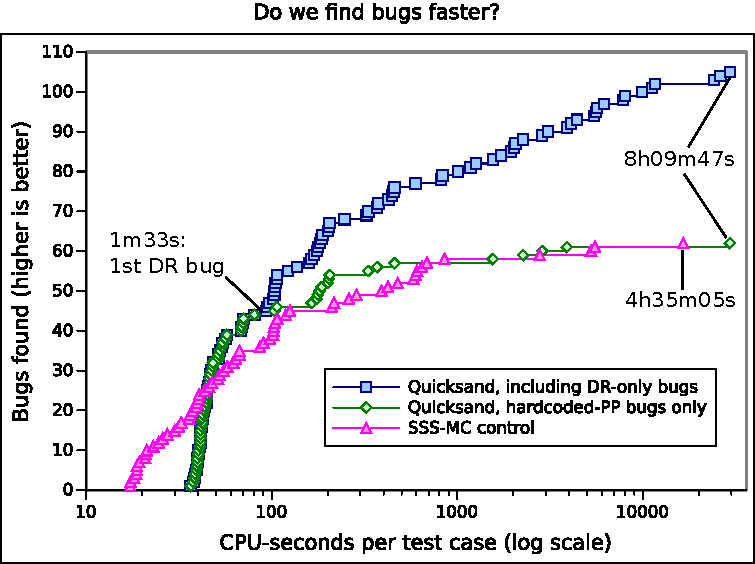
\includegraphics[width=0.48\textwidth]{dowefindbugsfaster.pdf}
	\caption{Comparison of bug-finding performance
	by several configurations of \quicksand~and the SSS-MC control.
	\quicksand~finds 179\% as many bugs with data-race PPs.}
	\label{fig:dowefindbugsfaster}
\end{figure}

{\bf Finding the same bugs faster.}
To show that Iterative Deepening is effective even for MC domains without data races, such as message-passing distributed systems,
we ran the test suite with \quicksand~configured to explore only subsets of the hard-coded mutex PPs
(i.e., ignoring all data-race candidates)\footnote{
Because \quicksand~is not yet instrumented to subset hard-coded PPs beyond the 4 ways shown in Figure~\ref{fig:id},
we ran these tests for 2.5 hours on 4 CPUs each.
Future work could parallelize QS-no-DR-PPs further; see \sect{\ref{sec:future}}.}.
%
The line QS-no-DR-PPs represents this experiment.
Even though SSS-MC mostly catches up to it by the end of the 10-hour budget,
QS-no-DR-PPs finds many more of the bugs much sooner.
From this we conclude that for smaller arbitrary CPU budgets,
Iterative Deepening is likely to find bugs SSS-MC will miss,
and for more ambitiously-sized tests,
programmers can be more confident in the verification provided when \quicksand~times out with no bug found.
%We conclude that for smaller arbitrary CPU budgets, especially less than 1 hour,
%Iterative Deepening is likely to find bugs SSS-MC will miss.
%Moreover, it is also easy to imagine scaling up the size of each test case to test ,
%using more threads or longer sequences of API calls.
%We hope that is compelling even to users willing to spend many CPU-hours on testing.
%These results show explicitly that for arbitrary CPU-time budgets

%Note that even users willing to spend 10 CPU-hours should find this ``early advantage'' compelling:

{\bf Finding new data-race bugs.}
Though state-of-the-art MCs preempt only on synchronization events, many serious concurrency bugs are caused by data races leading to corrupted shared state.
The line QS-DRs represents our ``no holds barred'' \quicksand~tests,
with dynamically-discovered data-race PPs enabled:
we quickly pull ahead of SSS-MC, and ultimately conclude with 179\% as many bugs in total.
The break-even point is at a negligible 90 seconds.

Furthermore, we plotted another line from this dataset, QS-no-DR-bugs,
which represents only the bugs found in state spaces without data-race PPs (like QS-no-DR-PPs, but even when data-race PPs are enabled).
Intuitively, this line shows that for programs with only benign data races,
\quicksand~can afford the extra overhead of verifying them while still slightly edging out SSS-MC.
%\footnote{The initial perfect overlap between QS-DRs and QS-no-DR-bugs indicates how long it takes before the first data-race bug is found.}
%even after the extra overhead of verifying them, \quicksand~still slightly edges out SSS-MC

\begin{table*}[t]
	\begin{center}
		%\small
	\begin{tabular}{r|c||c|c|c||c|c|c|c|c}
		% TODO: Make the "bugs" left half of this graph into a bar graph.
		& {\bf Num.} & {\bf SSS-MC} & {\bf QS} & {\bf DR-only} & {\bf Total} & {\bf Untested} & {\bf Malloc-} & {\bf Nondet.} & {\bf Nondet.} \\
		{\bf Test name} & {\bf tested} & {\bf bugs} & {\bf bugs} & {\bf bugs} & {\bf DR PPs} & {\bf DR PPs} & {\bf recycle DRs} & {\bf DR PPs} & {\bf DR bugs} \\
		\hline
		{\bct		} & 79	& 7	& 11	& 4	&	&	& 65	&	& 4	\\
		{\tej		} & 79	& 14 	& 25	& 11	&	&	& 471	&	& 6	\\
		{\mxtest	} & 79	& 1	& 10	& 9	&	&	& 7	&	& 1	\\
		{\paradise	} & 79	& 10	& 17	& 7	&	&	& 268	&	& 3	\\
		{\paraguay	} & 79	& 4	& 12	& 9	&	&	& 188	&	& 0	\\
		{\rwldgr	} & 79	& 26	& 30	& 3	&	&	& 157	&	& 3	\\
		\hline
		{\prisema	} & 59	&	&	&	&	&	& 0	&	&	\\
		{\alarmsimul	} & 44	&	&	&	&	&	& 37	&	&	\\
		{\waitsimple	} & 52	&	&	&	&	&	& 57	&	&	\\
		\hline
		{\bf Total}	& 629	&	&	&	&	&	& 1250	&	&
	\end{tabular}
	\end{center}
	\caption{Summary of number and types of bugs found by each test case.
		SSS-MC is the control; QS is \quicksand.
		``DR-only'' counts among \quicksand's bugs how many required data-race PPs to expose (\sect{\ref{sec:eval-sssmc}}).
	``Nondeterministic DRs'' counts among the DR-only bugs how many candidates required MC integration to identify (\sect{\ref{sec:eval-falseneg}}).
		TODO: more explanation}
	\label{tab:drbugs}
\end{table*}

\begin{figure}[t]
	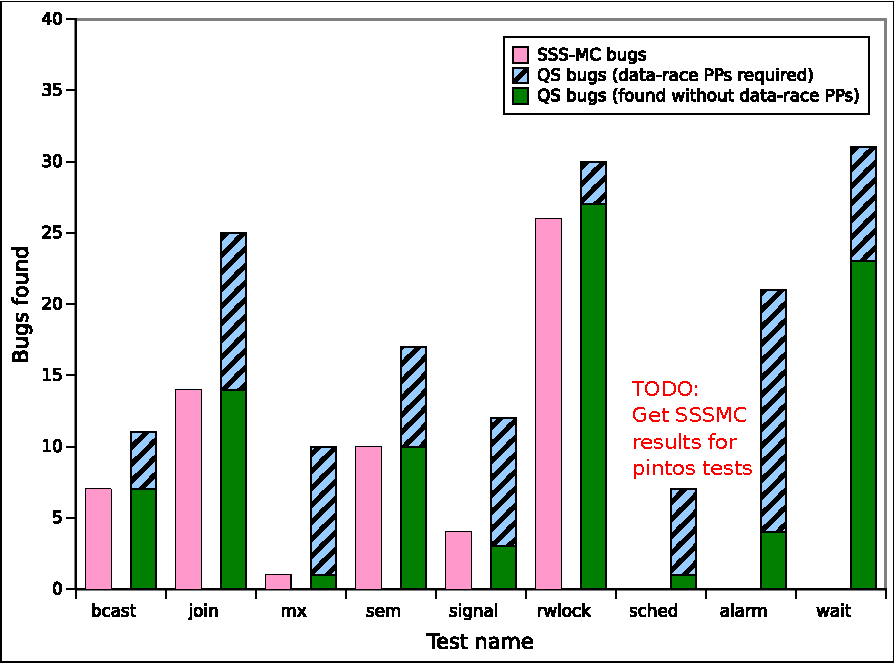
\includegraphics[width=0.48\textwidth]{bargraph.pdf}
	\caption{{\bf TODO:} Is this graph productive to include in the paper? Or should I just leave the numbers in table format (the left half of Table~\ref{tab:drbugs})?}
	\label{fig:bargraph}
\end{figure}

%Figure~\ref{fig:bargraph}
The left half of Table~\ref{tab:drbugs}
breaks down the number and types of bugs found by each test case.
% The astute observer will note that the sum of all types of failures observed is more than the total number of data-race bugs...
%TODO CAMREADY: Run a mutex expt where "all atomic instrs" are PPs. See how many bugs are missed anyway.
% Wwe re-ran the \mxtest control experiment with \landslide~hard-coded to preempt on any atomic instruction
% (as well as on the mutex API boundaries).
% Still, this smarter configuration for SSS-MC found only 99999999999 bugs of \quicksand's 13.
In \mxtest~in particular, the control experiment found dramatically fewer bugs (just 1),
even compared to the other test cases\footnote{
% "Aren't all lock impls assembly?" "Yes, but this one was ALL assembly."
	The one bug SSS-MC found was in a fully-assembly lock implementation. {\tt yield()}'s return value clobbered a value stored in {\tt \%eax}, which could lead to a failure after two repeated contentions. Preempting only on {\tt yield()} (in the contention loop) was sufficient.}.
%Intuitively, this is due to our control experiment being able to preempt only on the boundaries of the API which
%Though for many applications of MC, assuming a correct lock implementation is sufficient,
Though it suffices for many applications of MC to assume correctly-implemented locks,
we consider this strong evidence that any verification of low-level synchronization code must incorporate data-race PPs.

{\bf Partial verification.}
When a state space times out, the user may prefer a brief summary of what parts of the test were verified, rather than writing off all the CPU time as a waste.
Beyond using the state space estimator to guess the percent coverage,
we know of no approach to quantify the probability
that a bug would be exposed by an untested interleaving.
\quicksand~does not attempt any such quantitative guarantee,
but can at least report which subsets of PPs produced state spaces that did complete in time.

The SSS-MC control experiment timed out in 10 hours on 77 tests.
Among these, \quicksand~found data-race bugs in 15.
For the other 62, we counted the number of state spaces \quicksand~was able to complete and the number of unique PPs among them.
In three cases, \quicksand~also failed to complete anything; beyond these,
between 1 and 253 state spaces were completed, with a mean of 58.9 and median of 29.
Between 0 and 233 unique PPs were tested among some completed subsets, with a mean of 27.2 and median of 7.5.
These completions guarantee that, if the test case could expose a bug,
% Justify implicit hypothesis: Sync PPs + DR PPs = all possible relevant PPs.
it would only be found by a new data-race PP not discovered yet, or by a superset combination of PPs not reached.

%Hence, in Table~\ref{tab:drbugs} we count how often \quicksand~uncovered a bug only in state spaces which included data-race PPs, while
%
%In Table~\ref{tab:allbugs} ....

%%%%%%%%%%%%%%%%%%%%%%%%%%%%%%%%%%%%%%%%%%%%%%%%%%%%%%%%%%%%%%%%%%%%%%%%%%%%%%%%

\subsection{Avoiding false positive data-race candidates}
\label{sec:eval-falsepos}
% Though we mechanically verify whether each data race candidate leads to a bug, each new PP can increase combinatorially..... obviously wish to avoid...

Beyond finding new bugs with data-race PPs, we evaluated \quicksand's performance in classifying data-race candidates in two ways.

{\bf Suppressing ``malloc-recycle'' false positives.}
In \sect{\ref{sec:recycle}} we showed the soundness of suppressing data race reports between two heap accesses when the surrounding memory was re-allocated in between.
In Table~\ref{tab:drbugs}, the column ``Malloc-recycle DRs'' shows the total number of such data-race candidates for each test case.
In total, 1250 data-races fit the malloc-recycle pattern across all tests,
only 69 of which were observed to avoid the re-allocation in an alternate interleaving.
Our proof in \sect{\ref{sec:recycle}} guarantees the safety of pruning all 1181 other state spaces.

Among the 69 true data-races which initially fit the malloc-recycle pattern,
none of them exposed a new bug when used as a PP.
This shows that for other data-race tools,
suppressing malloc-recycle candidates may be a productive heuristic,
even if unsound without Iterative Deepening.
However, \quicksand~was able to correctly identify the 69 violations of that heuristic among 30 distinct tests,
and fall back to classifying them with DPOR,
which we consider a much stronger verification.

{\bf Full verification.}
For 153 of our 629 tests, \quicksand~was able to provide the total verification guarantee described in \sect{\ref{sec:totalverif}}.
In Figure~\ref{fig:totalverif} we plot the cumulative distribution of \quicksand's total verifications before a given elapsed CPU-time.
Among these, 36 tests contained no data-race candidates whatsoever, 
so the same verification could be provided by SSS-MC.
We plot these for comparison,
according to the time taken by that test's SSS-MC control experiment,.
When a test can be totally verified without any data-race PPs,
\quicksand~will be slower than SSS-MC due to redundant work (\sect{\ref{sec:future}}).
Of course, using data-race PPs increases our capacity for total verification by 4.25x.

\begin{figure}[t]
	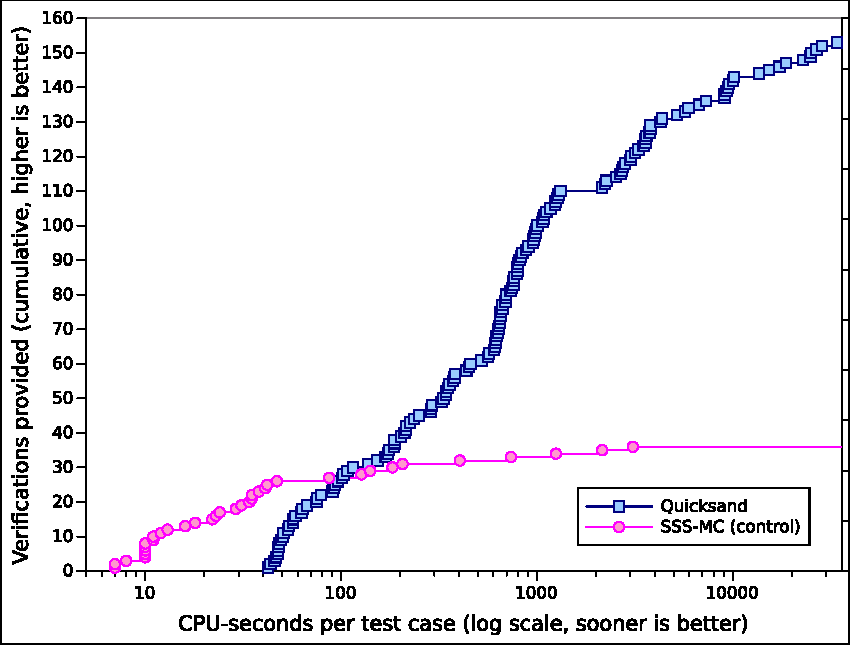
\includegraphics[width=0.48\textwidth]{totalverifs.pdf}
	\caption{Cumulative distribution of tests \quicksand~fully verified (\sect{\ref{sec:totalverif}}).
	Some tests had no data-race candidates, and hence could also be verified by SSS-MC.}
	\label{fig:totalverif}
\end{figure}

% TODO: Figure out how to visualize how many unique data race PPs were verified, and how many remained as unclassified false positives

%%%%%%%%%%%%%%%%%%%%%%%%%%%%%%%%%%%%%%%%%%%%%%%%%%%%%%%%%%%%%%%%%%%%%%%%%%%%%%%%

\subsection{Finding nondeterministic data-race candidates}
\label{sec:eval-falseneg}
Some memory accesses may be hidden in a control flow path that requires a nondeterministic preemption to be executed.
In such cases, a single-pass dynamic data-race detector
%could not achieve the coverage necessary
would fail
to identify a racing access pair as a candidate to begin with.
%
We counted how many such data-races, used as PPs, led to \quicksand~finding new bugs,
thereby making them {\em false negatives} of the single-pass approach.
We classified each data-race candidate according to whether \landslide~had reported them during the first interleaving, before any backtracking or preempting: if so, they were {\em deterministic data races} (hence could be found by single-pass).

To ensure a fair comparison, we disabled \landslide's {\em false-positive}-avoidance techniques during this experiment.
For example, we reported malloc-recycle data races during the first interleaving as {\em deterministic}, as a single-pass analysis must,
rather than waiting until future interleavings to confirm them (as explained in \sect{\ref{sec:recycle}}).

TODO: Present results.

At first, it might seem unfair to compare the data race bugs \quicksand~finds (10 CPU-hours)
against the candidates found by a prior work's single execution (less than a minute).
We argue this comparison is meaningful because prior work data-race tools %, being not integrated with a MC,
are not intended to discover new data race candidates under subsequent runs. %before discovering any initial candidates.
Running a data-race tool repeatedly for 10 CPU-hours could potentially uncover some of these false negatives at random,
but stress testing's comparative problem with achieving reliable coverage is already well-understood
\cite{chess-icb,gambit}.
This experiment also suggests that
other replay-based data-race tools \cite{racefuzzer,portend} should be configured to use the same sort of feedback loop as Iterative Deepening (\sect{\ref{sec:related-dr}}).
%i.e., discovering transitively-reachable data races while testing initial ones.
%although that would still not simultaneously be able to provide total verifications.
% TODO: read gambit paper


% Figure out concretely what the data race tricks are that we do, so we can claim them as contributions in the paper. Then ACTUALLY EVALUATE THEM.
%         - Speculative DR PPs.
%                 Not a heuristic, rather how to make it work at all to begin with.
%                 (Cite MS thesis, claim on backwards explorating finding bugs faster)
%         - Free/re-malloc to eliminate some false positives. See #193.
%                 Measure how many false positives are eliminated.
%                 Check, ofc, to make ABSOLUTE SURE, that no bugs missed w/ this trick.
%                         If there are, it could be because of the implementation
%                         bug described in #193.
%         - Using tid/last_call filtering because whole stack traces are too expensive.
%                 Moderately optional, 1st priority since theoretically interesting:
%                 Turn on/off and measure how resulting DR bug #s change.
%         - Optional: Reprioritizing DRs based on "confirmed" / "suspected"
%                 Shouldn't be hard just make ID wrapper print "s" or "c"!
%                 Is it helpful for ID to put priorities on DR PPs?
%                         Test by inverting the priority and see if fewer buges are found.
%         // Super optional to talk about. Probably not worth the time.
%         // - "Too suspicious" (during init/destroy)
%         //      (Cite eraser, section 2.2)

%%%%%%%%%%%%%%%%%%%%%%%%%%%%%%%%%%%%%%%%%%%%%%%%%%%%%%%%%%%%%%%%%%%%%%%%%%%%%%%%

\section{Discussion}
\label{sec:future}

In this section, we discuss \quicksand's limitations and opportunities for future improvement.

% TODO CAMREADY: Measure how much subset overlap there is.
{\bf Avoiding redundant work.}
When we extend a small state space with more PPs, the new state space is guaranteed to test a superset of thread interleavings compared to the old one.
Any interleaving which does not preempt threads on any of the new PPs will be repeated work.
Because we prioritize completing small state spaces before extending them with more PPs,
the superset state spaces we run later will repeat each branch of their already-completed subsets.
%
%We measured the proportion of repeated work among completed state spaces across our test suite;
%on average, {\bf \large 999\%} of the interleavings in each test were repeated, with some tests as high as {\bf \large 9999\%}.

This repeated work can cause Iterative Deepening to be slower than SSS-MC to find certain bugs,
for example, if both {\tt mutex\_lock} and {\tt mutex\_unlock} preemptions together would expose a bug, but not either alone.
Similarly, when pursuing total verification (\sect{\ref{sec:totalverif}}),
if the state space resulting from preempting on every instruction could be completed,
an SSS-MC tool such as \cite{spin} might achieve that verification faster,
as Iterative Deepening will test many subsets of data-race PPs first.
Predicting whether each still-untested interleaving will uncover new PPs is not straightforward,
but we believe future implementations of Iterative Deepening could incorporate cross-job memoization
to prune some or all of this repeated work.

{\bf Finer-grained PP subsets.}
% TODO: update these numbers
\quicksand~was able to partially guarantee safety in 97\% of tests with large maximal state spaces.
However, in 2 tests, no more than the minimal state space could be verified,
and in 3 other tests, not even that much.
Larger state spaces often result from finer-grained locking,
which can indicate a more intricate concurrent algorithm or an unnecessarily complicated design.
Such programs may require even more rigorous verification than a program with a single global lock.
%Hence these corner cases are important to consider for future work.
While this work used {\tt within\_function} (\sect{\ref{sec:landslide}}) {\em statically} to restrict where PPs could arise in advance of the test,
we envision future Iterative Deepening implementations could incorporate this method to {\em dynamically} subset PPs further,
making partial verification of such large tests possible.
%enabling partial verification of such large tests. % if need space
%Because our current implementation does not avoid repeated interleavings across state spaces,
%as discussed above,
%we were limited to a small number of very basic PP subsets to statically seed the exploration

%{\bf Small test cases.}

{\bf Partial verification.}
We are not the first to provide a partial verification guarantee when timing out on too-large state spaces (\sect{\ref{sec:eval-sssmc}}).
While we guarantee safety when preempted on certain combinations of PPs,
CHESS
guarantees safety under no more than a certain number of preemptions \cite{chess-icb}.
%according to the maximum bound reached in the time limit.
We imagine these two guarantees could be each be useful to developers in different scenarios,
and are presently working to combine the two approaches to provide both at once.
One benefit of our technique is that {\tt within\_function}-based Iterative Deepening (discussed above)
would enable expert developers to configure custom subsets of PPs they are most interested in verifying,
according to which modules of a codebase they wish to test.

Likewise, for test cases where full verification is not computationally feasible,
the state spaces associated with many data-race candidates will time out.
We cannot guarantee that those races are false positives or benign, even though no bug was found.
% FIXME: You need a separate table counting only the state spaces WITHOUT BUGES.
In the ``Untested DR PPs'' column of Table~\ref{tab:drbugs}, we count the number of such unverified candidates from each test case.
For a more formal treatment of these cases, we refer the reader to the {\em k-witness harmless} metric introduced by \cite{portend},
which could be combined with Iterative Deepening in future work.
% Future work: Add parallel DPOR so you can fill your spare CPUs when there are fewer than the max number of jobs.
